\section{Software-Verzeichnisse und Paketverwaltung}
\label{sec:paketverwaltung}
% TODO noch mehr schreiben sollte auf 3 Seiten kommen
Im Gegensatz zur Versionsverwaltung verwaltet die Paketverwaltung keinen Code und dessen Änderungen, sondern fertige Softwarepakete, welche von Entwicklern erstellt und in einem Software-Verzeichnis abgelegt werden.
Inhalt eines Pakets können beispielsweise standardisierter Code von Software Modulen sein oder kompilierter Code.
Zusätzlich werden in einem Paket Metadaten gespeichert.
Diese Metadaten können beispielsweise eine Beschreibung, Version, Abhängigkeiten und Autoren des Paketes enthalten.
Sie lassen sich aus dem Paket mithilfe des Paketverwaltungssystems auslesen oder über APIs des Software-Verzeichnisses abrufen.
Außerdem übernimmt das Paketverwaltungssystem das Installieren und meistens auch das Aktualisieren und Deinstallieren von Paketen.
Zusätzlich wird das System verwendet, um fehlende Abhängigkeiten von Paketen automatisch zu installieren \autocite{spinellis_package_2012}.

In dieser Arbeit wird auf zwei Software-Verzeichnisse eingegangen.
Zum einen wird auf \gls{pypi} eingegangen, welches das Verzeichnis für Python ist und von der Paketverwaltung \emph{pip} verwendet wird.
Zum anderen wird auf \gls{cran} eingegangen, welches das Verzeichnis für R ist.
In \gls{pypi} sind aktuell mehr als 500.000 unterschiedliche Projekte mit über 5 Millionen Veröffentlichungen verfügbar \autocite{python_software_foundation_pypi_2024}.
Im Gegensatz dazu sind in \gls{cran} aktuell mehr als 20.000 Pakete verfügbar \autocite{cran_team_comprehensive_2024}.

\subsection{PyPI}
\label{subsec:paketverwaltung_pypi}
\gls{pypi} hat zu Beginn des Jahres 2024 ein \gls{pep} veröffentlicht, welches die Verifizierung von Daten auf \gls{pypi} beschreibt \autocite{python_software_foundation_pep_2024}.
In dem \gls{pep} werden Änderungen an der API beschrieben, welche zum Hochladen von Paketen genutzt wird, um sogenannte \glqq Attestation objects \grqq{} zu unterstützen, in denen digitale Signaturen enthalten sind.
Das Ziel ist es Verifizierte Daten auf \gls{pypi} zu ermöglichen, sodass Anwender direkt erkennen können, ob die Daten vertrauenswürdig sind.
Aktuell wird dieses \gls{pep} umgesetzt, wodurch es zu vielen Änderungen in der API und auch in der Weboberfläche von \gls{pypi} kommt.
Außerdem sind noch nicht alle Daten über die APIs erreichbar und es ist auch aktuell nicht über die API erkennbar, ob es sich um verifizierte oder nicht verifizierte Daten handelt.
Ein Beispiel für verifizierte Daten sind Links, beispielsweise auf GitHub.
Diese Links werden von \gls{pypi} als verifiziert angesehen, wenn der Upload des Paketes auf \gls{pypi} über eine GitHub Action erfolgt.
Außerdem werden die Personen als verifiziert dargestellt, welche in \gls{pypi} als Owner oder Betreuer des Pakets eingetragen sind, sie haben somit einen Account bei \gls{pypi}.
Owner können dabei alle Änderungen am \gls{pypi} Projekt vornehmen und Betreuer können neue Versionen des Paketes veröffentlichen \autocite{ingram_deprecate_2023}.
In \autoref{fig:pypi_verified_unverified_details} ist dargestellt, wie verifizierte und unverifizierte Daten auf \gls{pypi} dargestellt werden.
Die dargestellten GitHub Statistiken werden dabei von \gls{pypi} ermittelt und nicht über APIs ausgegeben.
Das Ziel von \gls{pypi} ist es, dass alle Daten verifiziert werden können und keine Daten mehr in der unverifizierten Form vorliegen.

\begin{figure}
    \centering
    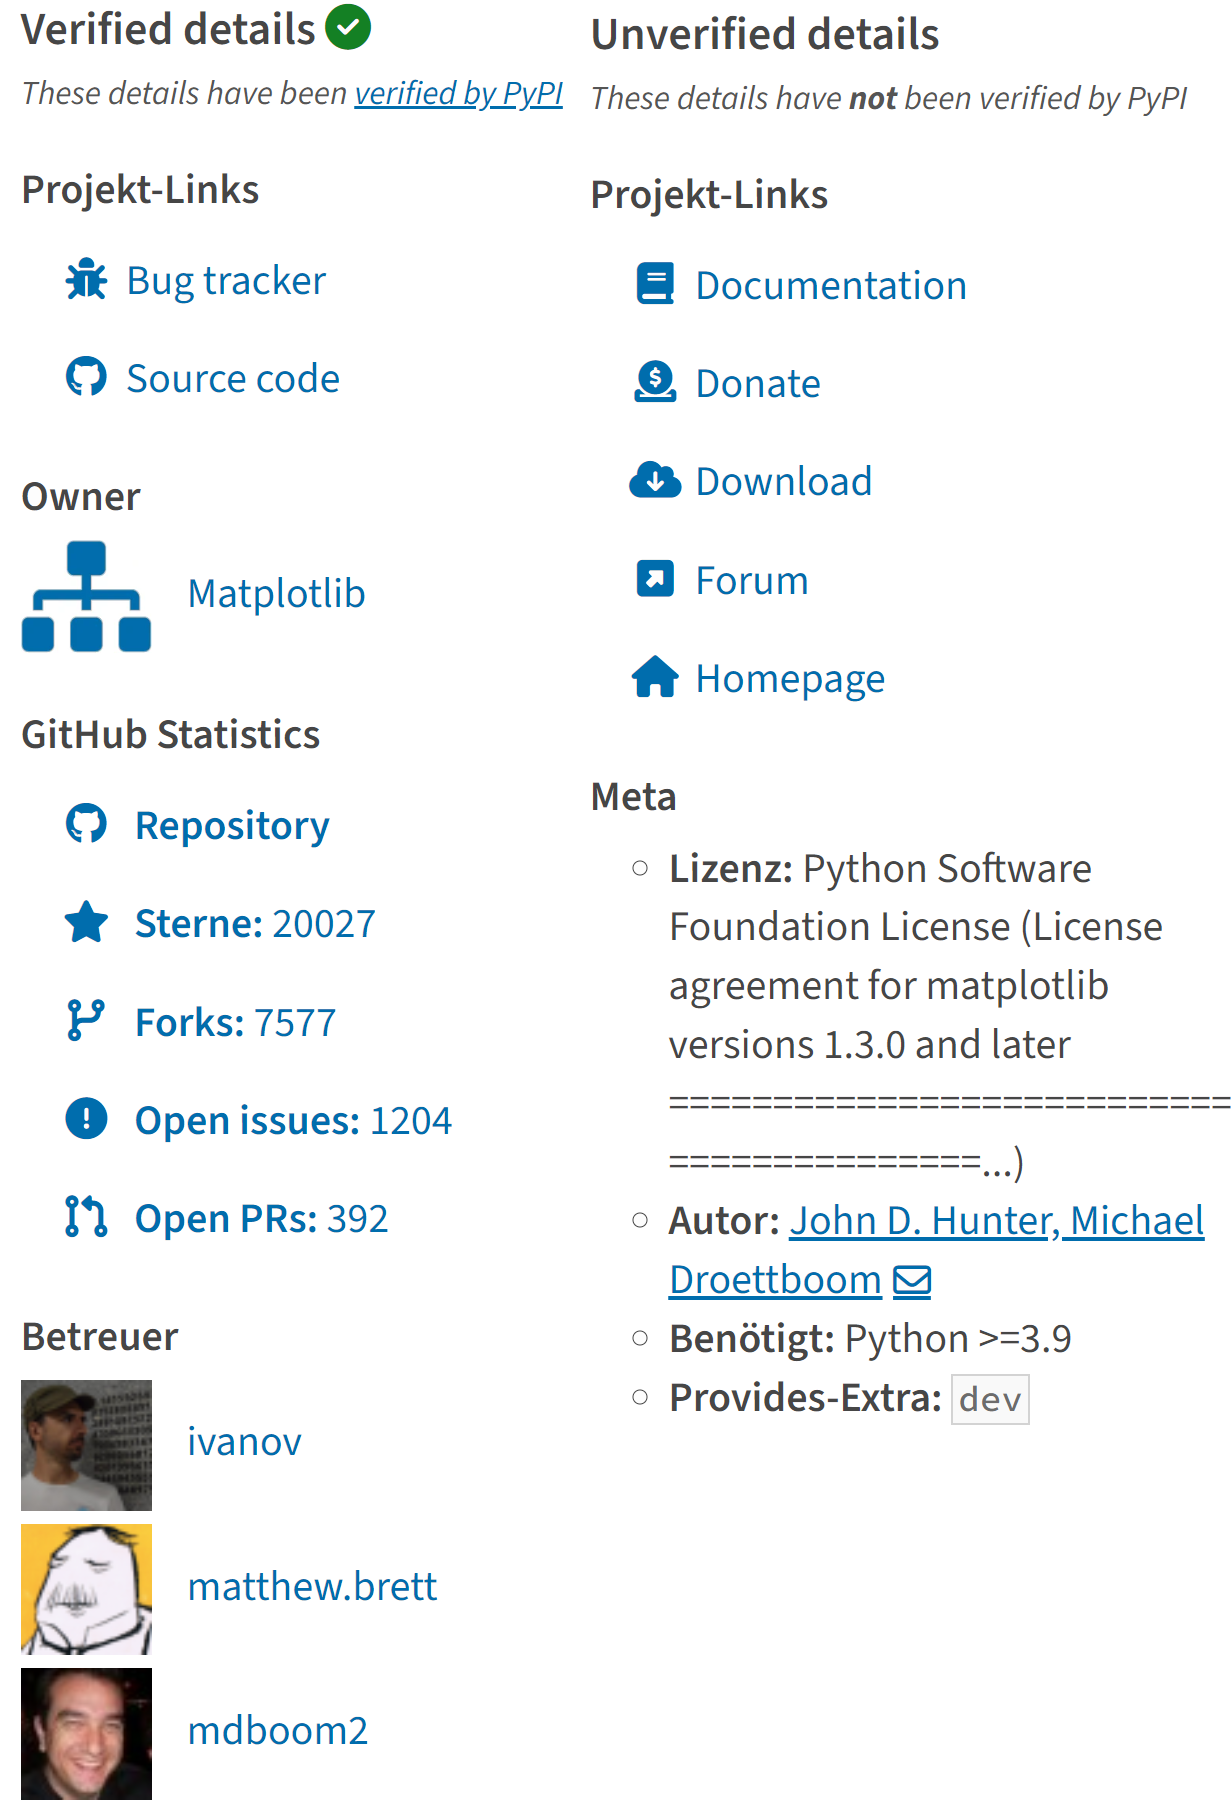
\includegraphics[width=\textwidth]{bilder/pypi.png}
    \caption{\gls{pypi} Verifizierte und unverifizierte Daten}
    \label{fig:pypi_verified_unverified_details}
    \small
    Die Abbildung stellt die verifizierten und unverifizierten Daten des Pakets \emph{matplotlib} auf \gls{pypi} dar \autocite{python_software_foundation_pypi_2024}.
\end{figure}

\gls{pypi} bietet verschiedene APIs und Quellen an, um die Daten der Pakete abzufragen.
Im Folgenden werden auf einige der Zugriffsmöglichkeiten eingegangen, welche mit Ausnahme der BigQuery alle in dieser Arbeit verwendet werden.

\subsubsection*{JSON API}
\label{subsubsec:pypi_json_api}
% TODO Die nicht verifizierten Daten stammen aus der Python toml (stammen die Daten wirklich alle aus der toml?) Falls ja das erwähnen und erklären, dass die Daten direkt von dem Python paket stammen und pypi diese nur durchreicht
Die JSON API ist die bevorzugt zu verwendende API von \gls{pypi} und bietet die Möglichkeit die Metadaten (Info) eines Pakets abzufragen.
Diese API ist nicht in der Anzahl der Anfragen beschränkt.
Dabei werden die Daten der neustens Version des Pakets zurückgegeben.
Die Werte der Metadaten stammen aus den Daten, welche beim Hochladen auf \gls{pypi} angegeben wurden.
Die Daten des ersten Uploads eines Releases werden dabei als Metadaten der Version gespeichert und bei weiteren Uploads dieser Version nicht überschrieben.

Inhalt der Metadaten sind beispielsweise die Autoren und Maintainer zuzüglich deren E-Mail-Adresse, die Beschreibung, Lizenz und Links zu unterschiedlichen Quellen Beispielsweise einem GitHub Repository \autocite{python_software_foundation_warehouse_2024}.
Die Beschreibung kann den Text aus der README-Datei des Pakets auf GitHub enthalten.
Es ist jedoch auch möglich eine eigene Beschreibung für \gls{pypi} anzugeben, sodass sich die README-Datei in GitHub und die Beschreibung auf \gls{pypi} unterscheiden können.
Die Metadaten werden von den Entwicklern des Pakets eingetragen.
In \autoref{fig:pypi_verified_unverified_details} sind einige der Metadaten des Pakets \emph{matplotlib} unter dem Punkt \glqq Meta\grqq{} dargestellt.
Weitere Daten sind unter dem Punkt \glqq Projekt-Links\grqq{} unter den verifizierten Details dargestellt.
Aktuell gibt die JSON API noch keine Auskunft darüber, ob die Daten verifiziert sind oder nicht die Weboberfläche stellt dies bereits dar.

Die Autoren und Maintainer aus den Metadaten müssen nicht den verifizierten Betreuern und Owner des Pakets auf \gls{pypi} entsprechen, da dies unterschiedliche Systeme sind.
Zum einen sind es die Benutzer, welche Rechte auf \gls{pypi} haben um das Paket dort anzupassen und zum anderen sind es die Personen, welche durch die Entwickler des Pakets angegeben werden.
Die Autoren und Maintainer können jedoch ebenfalls verifiziert sein, wobei dies über die API noch nicht abgefragt werden kann, jedoch in der Weboberfläche bereits für einige Pakete dargestellt wird.
Es gibt aktuell wenig Pakete, bei denen die Autoren verifiziert sind, ein Beispiel ist das Paket \emph{hololinked}, welches zum Zeitpunkt des Schreibens darüber verfügt.
\emph{Matplotlib} unterstützt dies aktuell noch nicht, wie in \autoref{fig:pypi_verified_unverified_details} dargestellt ist.
Die verifizierten Betreuer und Owner können aktuell nicht über die JSON API abgefragt werden, sondern müssen über die XML-RPC API abgefragt werden, welche im Folgenden erläutert wird.

\subsubsection*{PyPI XML-RPC}
\label{subsubsec:pypi_xml_rpc}
Die \gls{pypi} XML-RPC API ist eine veraltete API, welche jedoch noch genutzt werden kann, um einige Informationen zu den Paketen abzufragen.
Es wird empfohlen diesen API nicht mehr zu verwenden und auf den RSS Feed oder die JSON API umzusteigen \autocite{python_software_foundation_warehouse_2024}.
Dadurch ist die API stark limitiert in der Anzahl der möglichen Anfragen und auch die Abstände zwischen den Anfragen müssen relativ groß sein.
\gls{pypi} macht keine genauen Angaben darüber, wie viele Anfragen in welchem Zeitraum möglich sind.
Diese API ist jedoch die einzige Quelle, um die Betreuer und Owner eines Pakets abzufragen, ohne einen Web-Scraper einsetzen zu müssen.
Web-Scraping bezeichnet dabei das Extrahieren von Daten aus Webseiten, indem der HTML-Code der Webseite analysiert wird \autocite{richardson_beautifulsoup4_2024}.

Die Owner und Betreuer, welche über die API ausgegeben werden, enthalten den Benutzernamen auf \gls{pypi}, ein Vollname wird hierbei nicht ausgegeben.
Der Benutzername für die Betreuer des Pakets \emph{matplotlib} sind in \autoref{fig:pypi_verified_unverified_details} unter dem Punkt \glqq Betreuer\grqq{} dargestellt.
Aktuell stellt \gls{pypi} keine API bereit, um den Namen eines Benutzers abzufragen, sodass nur der Benutzername über eine API abgefragt werden kann \autocite{python_software_foundation_add_2024}.

\subsubsection*{BigQuery}
\label{subsubsec:pypi_bigquery}
Ebenfalls bietet \gls{pypi} über Google BigQuery einen Datensatz an, in dem alle Pakete mit ihren Versionen und Metadaten enthalten sind \autocite{python_software_foundation_warehouse_2024}.
BigQuery ist ein Dienst von Google, welcher auf der Infrastruktur der Google Cloud Plattform ausgeführt wird \autocite{google_bigquery_2024}.
Es ist möglich den kompletten Datensatz auf BigQuery in mehreren einzelnen CSV-Dateien herunterzuladen.
Dabei kann ausgewählt werden, welche Daten heruntergeladen werden sollen.

Nicht alle Metadaten, welche über die JSON API abgefragt werden können stehen in der BigQuery zur Verfügung.
Ebenfalls stehen nicht alle Daten der BigQuery in der JSON API zur Verfügung.
Die wichtigsten Daten sind in beiden Quellen enthalten.
So ist beispielsweise der Autor und Maintainer und deren E-Mail-Adressen in beiden Quellen enthalten.
Auch die Beschreibung, Version und Abhängigkeiten sind in beiden Quellen enthalten.
Die jeweiligen Daten, wie die Autoren eines Pakets, sind in beiden Quellen identisch.

\subsection{CRAN}
\label{subsec:paketverwaltung_cran}
\gls{cran} selbst bietet keine API an, um die Metadaten der Pakete abzufragen.
Jedoch gibt es das METACRAN-Projekt, welches eine Kollektion von kleinen Diensten für das \gls{cran}-Repository bereitstellt.
Eines dieser Dienste ist eine CouchDB, welche die Metadaten aller Pakete von \gls{cran} bereitstellt.
Eine CouchDB ist eine Apache Datenbank, welche nativ eine HTTP/JSON API bereitstellt \autocite{the_apache_software_foundation_apache_2024}.
Die Datenbank ist eine Kopie des \gls{cran}-Repository und wird regelmäßig aktualisiert \autocite{csardi_pkgsearch_2023}.
Die Ausgabe der API erfolgt in JSON und teilweise sind einzelne Felder in R formatiert.
